\documentclass[xcolor=dvipsnames, 8pt]{beamer} %
%\setbeamertemplate{navigation symbols}{}

\usetheme{SantaBarbara}

\definecolor{black}{HTML}{0A0A0A}
\definecolor{red}{HTML}{e00404} 
%\definecolor{violet}{HTML}{231A97}

%\definecolor{darkgreen}{HTML}{008000}
\definecolor{gold}{HTML}{FFD000}
\setbeamercolor{normal text}{fg=black,bg=white}
\setbeamercolor{alerted text}{fg=red}
\setbeamercolor{example text}{fg=black}
\setbeamercolor{palette primary}{fg=black, bg=gray!20}
\setbeamercolor{palette secondary}{fg=black, bg=gray!20}

\setbeamercolor{palette tertiary}{fg=white, bg=red!80}
\setbeamercolor{block title}{fg=black,bg=gold!40}
\setbeamercolor{frametitle}{fg=white, bg=red!80}
\setbeamercolor{title}{fg=white, bg=red!80}


\usepackage[utf8]{inputenc}

\usepackage{tightlist}
\usepackage{tikz, tikzsettings}
\usepackage{verbatim}
\usepackage{amssymb}
\usepackage{amsmath}
\usepackage{amsfonts}
\pdfmapfile{+sansmathaccent.map} % Fix done for making the talk in ubuntu.
\usepackage{algorithmic}
\graphicspath{{./}{./figures/}{./figures/presentation/}}

%\usepackage[version=4]{mhchem}
\usepackage{subcaption}
\usepackage[authoryear,round]{natbib}
%\usepackage{fancyvrb}
\usepackage{color}
\usepackage{colortbl}
\usepackage{xcolor}
%\usepackage{physics}
\usepackage{pgfplots}
\usepackage{ragged2e}
%\pgfplotsset{compat=newest} \pgfplotsset{plot coordinates/math parser=false}
%\usepackage{environ} \usetikzlibrary{decorations.markings}
%\usetikzlibrary{decorations.pathreplacing}
\usetikzlibrary{shapes,calc,spy, calc, backgrounds,arrows, fit, decorations.pathmorphing, decorations.pathreplacing, matrix}
%\usepackage[absolute,overlay]{textpos}
\usepackage{caption}
\usepackage{mpcsymbols}
\usepackage{graphicx}
%\usepackage[controls=true,poster=first]{animate}


\AtBeginSection[] {\frame<beamer>{\frametitle{Outline}   
	\tableofcontents[currentsection, currentsection]}
	\addtocounter{framenumber}{-1}}
	%
%{
%	\frame<beamer>{\frametitle{Outline}   
%	    \tableofcontents[currentsection,currentsubsection]}
		
%}
\newcommand{\calert}[1]{\textcolor{blue}{#1}}

\makeatother
\setbeamertemplate{footline}
{\leavevmode%
	\hbox{%
		\begin{beamercolorbox}[wd=.3\paperwidth,ht=2.25ex,dp=1ex,center]{author
		in head/foot}%
			\usebeamerfont{author in head/foot}\insertshortauthor
		\end{beamercolorbox}%
		\begin{beamercolorbox}[wd=.6\paperwidth,ht=2.25ex,dp=1ex,center]{title
		in head/foot}%
			\usebeamerfont{title in head/foot}\insertshorttitle
		\end{beamercolorbox}%
		\begin{beamercolorbox}[wd=.1\paperwidth,ht=2.25ex,dp=1ex,center]{date in
		head/foot}%
			\insertframenumber{} / \inserttotalframenumber\hspace*{1ex}
	\end{beamercolorbox}}%
	\vskip0pt%
}


\title{Case studies on hybrid modeling with applications to process optimization}
\date{October 26, 2021}
\author[Pratyush Kumar]{\large Pratyush Kumar,
James B. Rawlings}
\institute[UCSB]{
	\begin{minipage}{4in}
		\vspace{-10pt}
		\centering
		\raisebox{-0.1\height}{\includegraphics[width=0.25\textwidth]{UCSB_seal}}
		%\hspace*{.2in}
		%\raisebox{-0.5\height}{\includegraphics[width=0.25\textwidth]{jci_logo}}
	\end{minipage}
	\vspace{10pt}
	\newline
	{\large Department of chemical engineering}
	\vspace{10pt}
	\newline
	{\large TWCCC meeting}}

\begin{document}

\frame{\titlepage}

%\section{Background}


\begin{frame}{Hybrid process modeling}

	\begin{columns}
	\column{\textwidth}

	\begin{block}{Motivation}
		\begin{itemize}
		\item A dynamic model of the process is required in feedback
		control applications to achieve operational objectives. \pause
		\item Usual first principles based \textcolor{blue}{grey-box models are
		incomplete}, and \textcolor{blue}{machine learning methods can provide a
		flexible approach to improve the performance of the grey-box
		models} for use in real time optimization (RTO).
		\end{itemize}
	  \end{block}
	  \pause
	  \bigskip
	\begin{block}{Literature}
	  \begin{itemize}
	  \item Use neural networks to approximate some state dependent process
	  parameters \footnote[frame]{\cite{psichogios:ungar:1992}} or to
	  approximate specific functions, e.g, unknown reaction rate laws, vapor
	  liquid equilibrium relationships,
	  \footnote[frame]{\cite{lovelett:avalos:kevrekidis:2019,
	  chen:ierapetritou:2020, bangi:kwon:2020}} in the grey-box models.	
	  \end{itemize}
	\end{block}
  
\end{columns}
\end{frame}

\begin{frame}{Chemical reactor example}

	\centerline{\resizebox{0.7\textwidth}{!}{\input{cstropt}}}
	\pause
	\begin{block}{Combine known \textit{structure} of the model with neural networks}
		\begin{equation*}
			\renewcommand{\arraystretch}{2}
			\begin{bmatrix} 
			\dfrac{dc_A}{dt} \\
			\dfrac{dc_B}{dt} \\
			\dfrac{dc_C}{dt}
			\end{bmatrix} = \begin{bmatrix}
	  \begin{array}{ccl}
			  \dfrac{Q_f(c_{Af} - c_A)}{V_R} &-& {\color{red} r_{1}} \\ 
			  -\dfrac{Q_fc_B}{V_R} &+& {\color{red} r_{1}} - 3\; {\color{red} r_{2}} \\
			  -\dfrac{Q_fc_C}{V_R} &+& \color{red}{r_{2}}
	  \end{array}
	  \end{bmatrix}
		  \end{equation*}
		  Often the reaction rate laws
		  ${\color{red}r_1}(c_j)$ and ${\color{red} r_2}(c_j)$ are unknown,
		  so approximate the rate laws with neural networks + data.
	\end{block}
\end{frame}

\begin{frame}{Sample training data}

	\begin{columns}

		\column{0.8\textwidth}
		\vspace{-0.1in}
		\begin{figure}
		  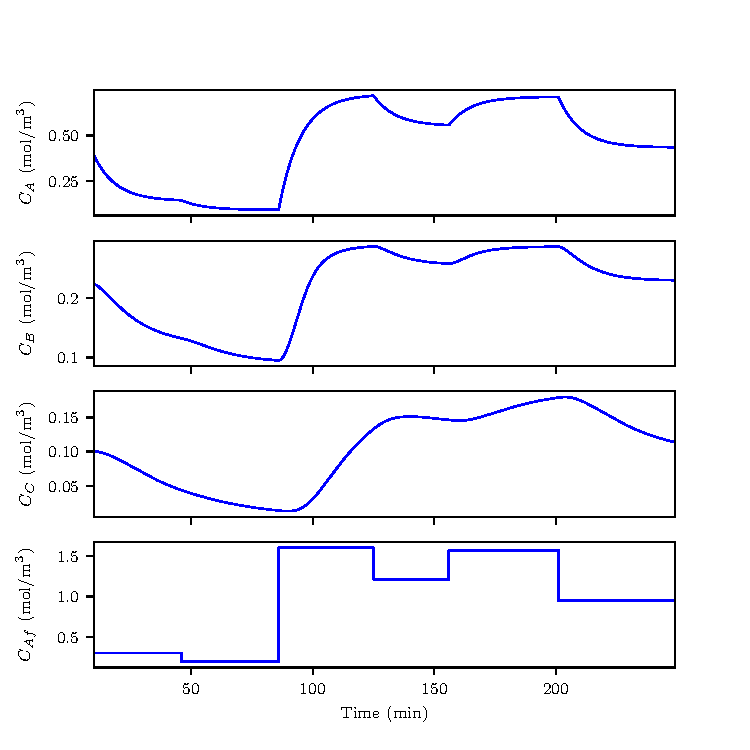
\includegraphics[page=1, height=0.8\textheight]{tworeac_plots.pdf}
		\end{figure}
	\end{columns}
	Data is generated by simulating the chemical reactor model. Train two types
	of models -- \alert{A black box neural network and hybrid model.}
\end{frame}

\begin{frame}{Errors in approximated rate laws by neural network}

	\begin{equation*}
	\textnormal{Error} = \dfrac{|\textnormal{Rate} - \textnormal{Rate}_{\textnormal{NN}}|}{\textnormal{Rate}}
	\end{equation*}
	\vspace{-0.1in}
		\begin{figure}
			\centering
		  \includegraphics[page=6, height=0.7\textheight, 
		  					width=0.48\textwidth]{tworeac_plots.pdf}
		  \includegraphics[page=7, height=0.7\textheight, 
		  				   width=0.48\textwidth]{tworeac_plots.pdf}
		\end{figure}
	The errors are \alert{below 10-20 $\%$} in the state-space visited
	in the training data. The approximation of the rate laws deteriorates
	outside the training data.
\end{frame}

\begin{frame}{Steady-state economic optimization}

	\begin{columns}
		\column{0.55\textwidth}
		\vspace{-0.1in}
		\begin{figure}
		  \includegraphics[page=5, height=0.7\textheight]{tworeac_plots.pdf}
		\end{figure}
	\column{0.4\textwidth}
	\begin{block}{RTO layer optimization problem}
		\begin{align*}
	\underset{u_s}{\textnormal{min}} & \ \ell(u_s, y_s) \leftarrow \textnormal{Economic Cost}\\
				x_s &= f(x_s, u_s) \\
				y_s &= h(x_s) \\
				\underline{u} \leq & u_s \leq \overline{u} 
		\end{align*}
	\end{block}
	\medskip
	\pause
	\begin{block}{Summary}
		\begin{itemize}
			\item Black-box models often result in unreliable
			optimization problems to solve subsequently.
			\item Hybrid models are more suitable for process optimization.
		\end{itemize}
	\end{block}
	\end{columns}
\pause

\begin{block}{Ongoing work}

\begin{itemize}
\item Examine the hybrid modeling approach on large, complex chemical
engineering examples for use in real-time optimization.
\end{itemize}

\end{block}

\end{frame}

\begin{frame}{References}
\bibliographystyle{abbrvnat}
\bibliography{articles,proceedings,books,unpub, resgrppub}
\end{frame}

\end{document}
